% TODO:
% - [x] Explain Ax = b
%    - [x] Add that you do work only until the last meaningful element
%    - [x] Add that you can only check for rows that are in your block, or block below if you are in the last row 
% - [x] Explain A = LU
% - [x] Explain LUx = b
% - [x] Explain Partial Selection Data Structure
% - [x] Explain Partial Selection Ax = b
% - [x] Explain Partial Selection A = LU
% - [x] Explain Partial Selection LUx = b
% - [x] Write about results
% - [ ] Correct grammar mess
\documentclass{article}
\usepackage{amsmath}
\usepackage{graphicx}
\usepackage[table]{xcolor}
\usepackage[T1]{fontenc}
\usepackage{algpseudocode}
\graphicspath{{images/}}
\title{List 5 report}
\author{Albert Kołodziejski}
\begin{document}
\maketitle
\section*{Without Partial Selection}
\subsection*{Data Structure}
We can safely assume that only cells that are colored can hold meaningful numbers when performing the algorithms. 
\begin{center}
    \begin{tabular}{| c|c|c | c|c|c | c|c|c |}
        \hline
        \cellcolor{blue!10} $a_{1,1}$ & \cellcolor{blue!10} $a_{1,2}$ & \cellcolor{blue!10} $a_{1,3}$ & \cellcolor{blue!10} $c_{1,4}$ & 0 & 0 & 0 & 0 & 0 \\
        \hline
        \cellcolor{red!10} $a_{2,1}$ & \cellcolor{red!10} $a_{2,2}$ &\cellcolor{red!10}  $a_{2,3}$ & \cellcolor{red!10} 0 & \cellcolor{red!10} $c_{2,5}$ & 0 & 0 & 0 & 0 \\
        \hline
        \cellcolor{green!10} $a_{3,1}$ & \cellcolor{green!10} $a_{3,2}$ & \cellcolor{green!10} $a_{3,3}$ & \cellcolor{green!10} 0 & \cellcolor{green!10} 0 & \cellcolor{green!10} $c_{3,6}$ & 0 & 0 & 0 \\
        \hline
        0 & 0 & \cellcolor{blue!25} $b_{4,3}$ & \cellcolor{blue!25} $a_{4,4}$ & \cellcolor{blue!25} $a_{4,5}$ & \cellcolor{blue!25} $a_{4, 6}$ & \cellcolor{blue!25} $c_{4,7}$ & 0 & 0 \\
        \hline
        0 & 0 & \cellcolor{red!25} $b_{5,3}$ & \cellcolor{red!25} $a_{5,4}$ & \cellcolor{red!25} $a_{5,5}$ & \cellcolor{red!25} $a_{5, 6}$ & \cellcolor{red!25} 0 & \cellcolor{red!25} $c_{5,8}$ & 0 \\
        \hline
        0 & 0 & \cellcolor{green!25}$b_{6,3}$ & \cellcolor{green!25} $a_{6,4}$ & \cellcolor{green!25} $a_{6,5}$ & \cellcolor{green!25} $a_{6, 6}$ & \cellcolor{green!25} 0 & \cellcolor{green!25} 0 & \cellcolor{green!25} $c_{6,9}$ \\
        \hline
        0 & 0 & 0 & 0 & 0 & \cellcolor{blue!50} $b_{7,6}$ & \cellcolor{blue!50}$a_{7,7}$ & \cellcolor{blue!50}$a_{7,8}$ & \cellcolor{blue!50} $a_{7,9}$ \\
        \hline
        0 & 0 & 0 & 0 & 0 & \cellcolor{red!50}$b_{8,6}$ & \cellcolor{red!50}$a_{8,7}$ & \cellcolor{red!50}$a_{8,8}$ & \cellcolor{red!50}$a_{8,9}$ \\
        \hline
        0 & 0 & 0 & 0 & 0 & \cellcolor{green!50}$b_{9,6}$ & \cellcolor{green!50}$a_{9,7}$ & \cellcolor{green!50}$a_{9,8}$ & \cellcolor{green!50}$a_{9,9}$ \\
        \hline

    \end{tabular}
\end{center}
It is also noteworthy that the majority of work done by the algorithms is done for one row, then another and so on. That's why I propose storing every color as a different Vector so that there will be fewer cache misses. The consideration here is to correctly interpret coordinates, as they are not the same as in the matrix.
\subsection*{Ax = b}
When developing the algorithm I have considered the following optimizations:
\begin{itemize}
    \item{There will be no operations for the last row}
    \item{When performing operations on rows, Let's say multiplying elements from the first row, and subtracting them from elements of the third row, we can stop when we reach the last meaning full element in the first row, so we will not do any operations on zeros}
    \item {When looking for elements that we want to turn into zeros, we can only look up to the last row in our block, or block below if we are in the last row}
\end{itemize}
Speed: O(n)\\
Memory: O(n)
\subsection*{A = LU}
When developing the algorithm I have considered the following optimizations:
\begin{itemize}
    \item{There will be no operations for the last row}
    \item{When performing operations on rows, Let's say multiplying elements from the first row, and subtracting them from elements of the third row, we can stop when we reach the last meaning full element in the first row, so we will not do any operations on zeros}
    \item {When looking for elements that we want to turn into zeros, we can only look up to the last row in our block, or block below if we are in the last row}
    \item {I can store $L$ and $U$ in the same matrix} 
\end{itemize}
Speed: O(n)\\
Memory: O(n)
\subsection*{LUx = b}
When developing the algorithm I have considered the following optimizations:
\begin{itemize}
    \item{Both $L$ and $U$ are triangular matrices, so computing $y$ and $x$ is very easy}
\end{itemize}
Speed: O(n)\\
Memory: O(n)
\newpage
\section*{With Partial Selection}
\subsection*{Data Structure}
Now we need to be careful because we can change rows, so the first row could end up in the last row. That's why I propose to store every row placed for 2 blocks plus one additional element. There should be ever more meaningful elements, and when we want to change a row on $2L + 2$ place, we can interpret the first element in the row as that, going around indexes if needed. Sadly that means we need a second structure to store $L$ as it will be no longer safe to store it in the same matrix as $U$.
\begin{center}
    \begin{tabular}{| c|c|c | c|c|c | c|c|c |}
        \hline
        \cellcolor{blue!10} $a_{1,1}$ & \cellcolor{blue!10} $a_{1,2}$ & \cellcolor{blue!10} $a_{1,3}$ & \cellcolor{blue!10} $c_{1,4}$ & \cellcolor{blue!10} 0 & \cellcolor{blue!10} 0 & \cellcolor{blue!10} 0 & 0 & 0 \\
        \hline
        \cellcolor{red!10} $a_{2,1}$ & \cellcolor{red!10} $a_{2,2}$ &\cellcolor{red!10}  $a_{2,3}$ & \cellcolor{red!10} 0 & \cellcolor{red!10} $c_{2,5}$ & \cellcolor{red!10} 0 & \cellcolor{red!10} 0 & 0 & 0\\
        \hline
        \cellcolor{green!10} $a_{3,1}$ & \cellcolor{green!10} $a_{3,2}$ & \cellcolor{green!10} $a_{3,3}$ & \cellcolor{green!10} 0 & \cellcolor{green!10} 0 & \cellcolor{green!10} $c_{3,6}$ & \cellcolor{green!10} 0 & 0 & 0\\
        \hline
        0 & 0 & \cellcolor{blue!25} $b_{4,3}$ & \cellcolor{blue!25} $a_{4,4}$ & \cellcolor{blue!25} $a_{4,5}$ & \cellcolor{blue!25} $a_{4, 6}$ & \cellcolor{blue!25} $c_{4,7}$ & \cellcolor{blue!25} 0 & \cellcolor{blue!25} 0 \\
        \hline
        0 & 0 & \cellcolor{red!25} $b_{5,3}$ & \cellcolor{red!25} $a_{5,4}$ & \cellcolor{red!25} $a_{5,5}$ & \cellcolor{red!25} $a_{5, 6}$ & \cellcolor{red!25} 0 & \cellcolor{red!25} $c_{5,8}$ & \cellcolor{red!25} 0\\
        \hline
        0 & 0 & \cellcolor{green!25}$b_{6,3}$ & \cellcolor{green!25} $a_{6,4}$ & \cellcolor{green!25} $a_{6,5}$ & \cellcolor{green!25} $a_{6, 6}$ & \cellcolor{green!25} 0 & \cellcolor{green!25} 0 & \cellcolor{green!25} $c_{6,9}$\\
        \hline
        0 & 0 & 0 & 0 & 0 & \cellcolor{blue!50} $b_{7,6}$ & \cellcolor{blue!50}$a_{7,7}$ & \cellcolor{blue!50}$a_{7,8}$ & \cellcolor{blue!50} $a_{7,9}$\\
        \hline
        0 & 0 & 0 & 0 & 0 & \cellcolor{red!50}$b_{8,6}$ & \cellcolor{red!50}$a_{8,7}$ & \cellcolor{red!50}$a_{8,8}$ & \cellcolor{red!50}$a_{8,9}$ \\
        \hline
        0 & 0 & 0 & 0 & 0 & \cellcolor{green!50}$b_{9,6}$ & \cellcolor{green!50}$a_{9,7}$ & \cellcolor{green!50}$a_{9,8}$ & \cellcolor{green!50}$a_{9,9}$ \\
        \hline
    \end{tabular}
\end{center}
Swapping rows of $A$ could take a long time so to avoid it we can use the vector of swaps, which simply stores indexes of rows, after swaps. So swaps are done on that vector, and when to get or set row $y$, we first change it to a local row after swaps.
\subsection*{Ax = b}
When developing the algorithm I have considered the following optimizations:
\begin{itemize}
    \item{There will be no operations for the last row}
    \item{When performing operations on rows, Let's say multiplying elements from the first row, and subtracting them from elements of the third row, we can stop when we reach the last meaning full element in the first row, so we will not do any operations on zeros}
    \item {When looking for elements that we want to turn into zeros, we can only look up to the last row in our block, or block below if we are in the last row}
    \item {When looking for a bigger element than the pivot, we can only look up to the last row in our block, or block below if we are in the last row}
\end{itemize}
Speed: O(n)\\
Memory: O(n)
\subsection*{A = LU}
When developing the algorithm I have considered the following optimizations:
\begin{itemize}
    \item{There will be no operations for the last row}
    \item{When performing operations on rows, Let's say multiplying elements from the first row, and subtracting them from elements of the third row, we can stop when we reach the last meaning full element in the first row, so we will not do any operations on zeros}
    \item {When looking for elements that we want to turn into zeros, we can only look up to the last row in our block, or block below if we are in the last row}
    \item {When looking for a bigger element than the pivot, we can only look up to the last row in our block, or block below if we are in the last row}
    \item {When looking for a bigger element than the pivot, we can only look up to the last row in our block, or block below if we are in the last row}
\end{itemize}
Speed: O(n)\\
Memory: O(n)
\subsection*{LUx = b}
When developing the algorithm I have considered the following optimizations:
\begin{itemize}
    \item{Both $L$ and $U$ are triangular matrices, so computing $y$ and $x$ is very easy}
\end{itemize}
Speed: O(n)\\
Memory: O(n)
\newpage
\section*{Results:}
\begin{center}
    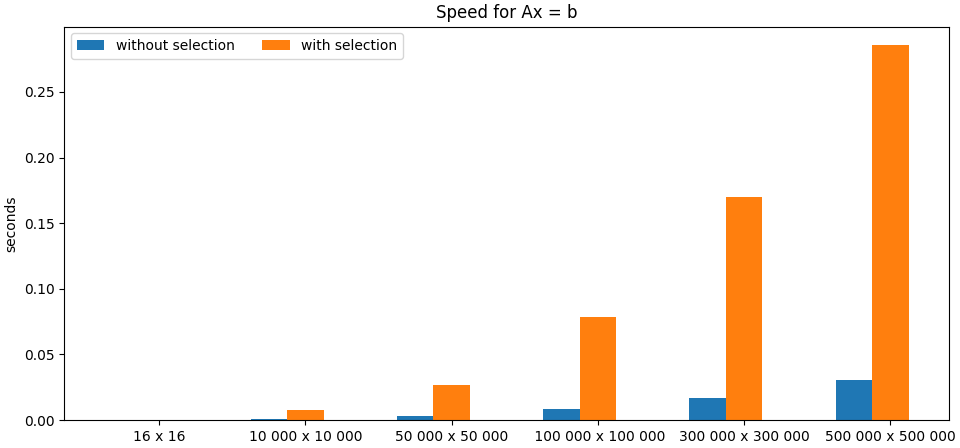
\includegraphics[scale=0.49]{Axb_Speed}
\end{center}
\begin{center}
    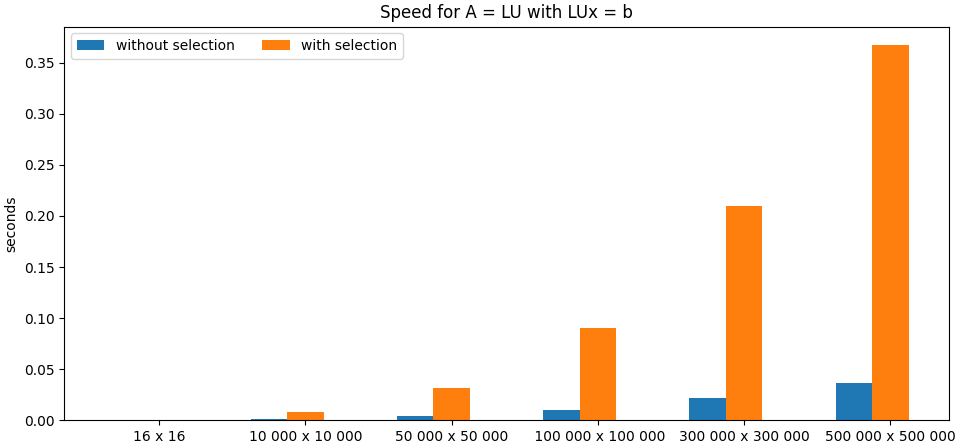
\includegraphics[scale=0.49]{LUxb_Speed}
\end{center}
\begin{center}
    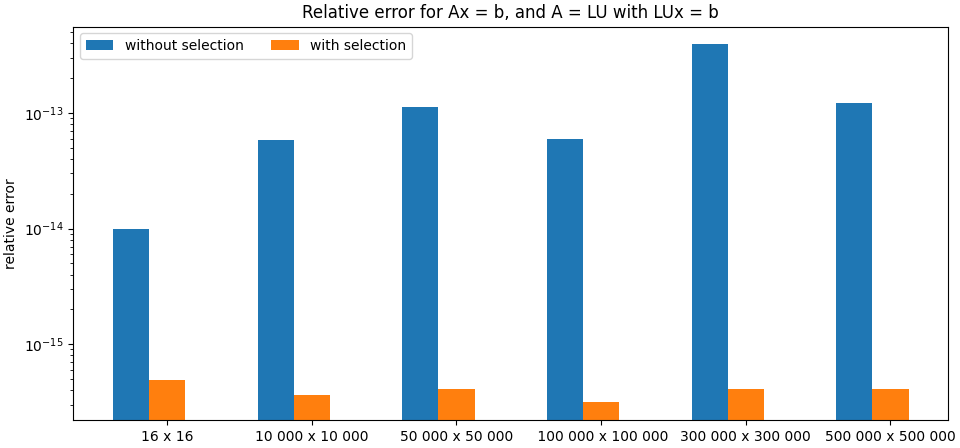
\includegraphics[scale=0.49]{Relative_error}
\end{center}
\end{document}